%%% Local Variables:
%%% mode: Xelatex
%%% TeX-master: t
%%% End:
\raggedbottom
\documentclass[finalformat,mathCMR]{WUSTthesis}% 盲审/正式用这个
%\documentclass[draftformat,mathCMR]{WUSTthesis}% 草稿用这个
%\raggedbottom

\usepackage{WUSTtils}% 所有其它可能用到的包都统一放到这里了，可以根据自己的实际添加或者删除。这样做主要是为了避免class文件过于臃肿。
%\usepackage[a4paper, margin=3.05cm]{geometry}
%\usepackage{mathfont}
\usepackage{amsmath,amssymb,amsfonts,bm}
\usepackage{listings}
\definecolor{codegreen}{rgb}{0,0.6,0}
\definecolor{codegray}{rgb}{0.5,0.5,0.5}
\definecolor{codepurple}{rgb}{0.58,0,0.82}
\definecolor{backcolour}{RGB}{245,245,245}

\lstdefinestyle{mystyle}{
    backgroundcolor=\color{backcolour},
    commentstyle=\color{codegreen},
    keywordstyle=\color{magenta},
    numberstyle=\tiny\color{codegray},
    stringstyle=\color{codepurple},
    basicstyle=\ttfamily\footnotesize,
    breakatwhitespace=false,
    breaklines=true,
    captionpos=b,
    keepspaces=true,
    numbers=left,
    numbersep=5pt,
    showspaces=false,
    showstringspaces=false,
    showtabs=false,
    tabsize=2
}
\lstset{style=mystyle, escapeinside=``}
\usepackage{graphicx}
\usepackage{ragged2e}
\newcolumntype{P}[1]{>{\RaggedRight\hspace{0pt}}p{#1}}
\newcolumntype{Z}{>{\centering\arraybackslash}X}
\usepackage{tabularx}
\usepackage{multirow}
\usepackage{newtxmath}
\DeclareSymbolFont{orilargesymbols}{OMX}{cmex}{m}{n}
\DeclareMathSymbol{\orisum}{\mathop}{orilargesymbols}{"50}
\renewcommand\sum\orisum
\renewcommand\geq\geqslant
\renewcommand\leq\leqslant
\RequirePackage[top=3cm, bottom=3cm, left=3cm, right=3cm, headheight=2.0cm, footskip=2.4cm,]{geometry}
\usepackage[font={small, stretch=1.5}, labelfont=bf, textfont=bf]{bicaption}
\captionsetup{labelsep=space}
\captionsetup[figure][bi-first]{name=图, font={small, stretch=1.5}, labelfont=bf, textfont=bf, justification=centering}
\captionsetup[figure][bi-second]{name=Figure, font={small, stretch=1.5}, labelfont=bf, textfont=bf, justification=centering}
\captionsetup[table][bi-first]{name=表, font={small, stretch=1.5}, labelfont=bf, textfont=bf, justification=centering}
\captionsetup[table][bi-second]{name=Table, font={small, stretch=1.5}, labelfont=bf, textfont=bf, justification=centering}
\usepackage[cal=cm]{mathalpha}
\setmainfont{Times New Roman}
\PassOptionsToPackage{no-math}{fontspec}
\usepackage{setspace}

%%% ============================================================
%%% 硕士论文适配：把模板默认的“博士”字样替换为“硕士”
%%% 模板默认定义在 WUSTthesis.cls 第 1396 / 1432-1434 行
%%% ============================================================
\makeatletter
\def\WUST@apply{硕士学位论文}
\renewcommand{\WUST@publication@title}{攻读硕士学位期间获得的学术成果}
\renewcommand{\WUST@patent@title}{攻读硕士学位期间申请的发明专利和其他成果}
\renewcommand{\WUST@project@title}{攻读硕士学位期间参加的科研项目}
\makeatother

\begin{document}
\begin{sloppypar}
%定义所有的eps文件在 figures 子目录下
\graphicspath{{figures/}}

% 生成封面，版权页，摘要
\frontmatter

%%% Local Variables:
%%% mode: Xelatex
%%% TeX-master: "../main"
%%% End:

%% ==================== 中文题目（≤30字） ====================
\ctitle{基于强化学习的两轮足机器人多步态运动控制与自适应调度方法研究}

%% ==================== 封面信息（请填写个人真实信息） ====================
\xuehao{【学号】} \schoolcode{10488}
\csubjectname{机械工程} \cauthorname{【姓名】}
\csupervisorname{【导师姓名】} \csupervisortitle{教授}
\defencedate{2027~年~5~月} \grantdate{}
\chair{}%
\firstreviewer{} \secondreviewer{} \thirdreviewer{}

%% ==================== 英文题目与封面信息 ====================
\etitle{Research on Multi-Gait Motion Control and Adaptive Scheduling Method for Two-Wheeled Legged Robot Based on Reinforcement Learning}
\edegree{Master of Science}
\esubject{Mechanical Engineering}
\eauthor{【Full Name】}
\esupervisor{Prof. 【Supervisor】}

%% ==================== 中文摘要（硕士约500字，宋体/Times New Roman 小四号，1.5倍行距） ====================
\cabstract{
    两轮足机器人以车轮为主要运动执行末端，兼具轮式移动的高效平稳性与足式结构的轻量化优势，在复杂地形巡检、物资运输与特种作业等场景具有广阔应用前景。然而，单一策略网络难以同时具备滚动行走、抬腿行走、跳跃、后空翻、抬腿上台阶与单腿平衡等多种步态能力，将多种步态直接纳入统一策略训练时，会产生灾难性遗忘、奖励冲突与局部最优等连续多任务学习的核心难题，严重制约策略的泛化能力与鲁棒性。

    针对上述问题，本文提出"分训-整合"的两阶段多任务强化学习框架。第一阶段，针对7类典型步态分别训练独立的步态专家策略网络，包括滚动行走（含侧向移动）、粗糙地形行走、抬腿行走、跳跃、后空翻、抬腿上台阶与单腿平衡，各专家在对应地形的专用环境中独立训练并达到验收标准；第二阶段，设计学习式统一调度器，该调度器以地形感知信息与机器人本体状态为输入，通过分层强化学习训练，在由平面、粗糙、碎石、台阶、独木桥、木桩与狭窄通道构成的混合地形统一环境中，自动选择或混合激活合适的步态专家，实现机器人按地形自适应切换步态：粗糙地形采用抬腿点足行走、低台阶抬腿跨越、高台阶跳跃上去、狭窄地形侧向移动、独木桥单腿平衡、木桩间隙跳跃通过。

    专家网络参数解耦从结构上规避了灾难性遗忘，各专家独立奖励函数与调度器高层目标分离缓解了奖励冲突，混合地形统一环境的细粒度评估与领域随机化抑制了局部最优。实验结果表明，所提框架能够使两轮足机器人在混合地形环境中完整遍历并自动切换步态，各步态专家在对应地形上均表现出良好的稳定性与鲁棒性，验证了"分训-整合"范式解决多任务强化学习整合难题的有效性。
}

\ckeywords{两轮足机器人；多任务强化学习；步态专家网络；学习式调度器；地形自适应步态切换}

%% ==================== 英文摘要（Times New Roman 小四号，1.5倍行距，首行缩进2个英文字符） ====================
\eabstract{
    The two-wheeled legged robot uses wheels as its primary locomotion end-effector, combining the high efficiency and stability of wheeled mobility with the lightweight advantages of legged structures, and holds broad application prospects in complex-terrain inspection, logistics transportation, and special operations. However, a single policy network can hardly master multiple gaits simultaneously, such as rolling walk, toe walk, jumping, backflip, stair leg lift, and single-leg balance. Directly integrating multiple gaits into one unified policy training inevitably gives rise to core challenges of continuous multi-task learning, including catastrophic forgetting, reward conflicts, and local optima, which severely restrict the generalization and robustness of the policy.

    To address these issues, this thesis proposes a two-phase "train-then-integrate" multi-task reinforcement learning framework. In the first phase, independent gait expert policies are trained separately for seven typical gaits, including rolling walk (with lateral movement), rough-terrain walking, toe walk, jumping, backflip, stair leg lift, and single-leg balance. Each expert is trained in a dedicated environment on its corresponding terrain and reaches an acceptance criterion. In the second phase, a learned unified scheduler is designed. Taking terrain perception information and the robot's proprioceptive state as inputs and trained by hierarchical reinforcement learning, the scheduler automatically selects or blends the appropriate gait experts in a unified mixed-terrain environment composed of flat, rough, rubble, stair, single-log bridge, stump, and narrow-passage terrains, enabling the robot to adaptively switch gaits according to terrain: toe-walking on rough terrain, stepping over low stairs, jumping onto high stairs, lateral movement in narrow spaces, single-leg balance on the single-log bridge, and jumping over stump gaps.

    The decoupled parameters of expert networks structurally avoid catastrophic forgetting; the separation of each expert's independent reward function from the scheduler's high-level objective alleviates reward conflicts; and fine-grained evaluation together with domain randomization in the unified mixed-terrain environment suppresses local optima. Experimental results show that the proposed framework enables the two-wheeled legged robot to traverse the mixed-terrain environment completely with automatic gait switching, and each gait expert exhibits favorable stability and robustness on its corresponding terrain, verifying the effectiveness of the "train-then-integrate" paradigm in solving the integration challenges of multi-task reinforcement learning.
}

\ekeywords{two-wheeled legged robot; multi-task reinforcement learning; gait expert network; learned scheduler; terrain-adaptive gait switching}

\makecover

% 生成目录
\clearpage
\pagestyle{tocpage} % 所有后续页使用 tocpage 样式
\thispagestyle{tocpage} % 强制当前页（目录第一页）生效
\tableofcontents
\clearpage

% 符号说明（必要时）
\begin{denotation}
\item[HRL] 分层强化学习（Hierarchical Reinforcement Learning）
\item[MoE] 专家混合模型（Mixture of Experts）
\item[PPO] 近端策略优化（Proximal Policy Optimization）
\item[SAC] 软演员-评论家算法（Soft Actor-Critic）
\item[N3PO] 带约束的自然策略梯度优化算法（Natural Policy Gradient with safety constraints）
\item[VMC] 虚拟模型控制（Virtual Model Control）
\item[SLIP] 弹簧负载倒立摆模型（Spring-Loaded Inverted Pendulum）
\item[CMDP] 约束马尔可夫决策过程（Constrained Markov Decision Process）
\item[MDP] 马尔可夫决策过程（Markov Decision Process）
\item[DRL] 深度强化学习（Deep Reinforcement Learning）
\item[MPC] 模型预测控制（Model Predictive Control）
\item[FSM] 有限状态机（Finite State Machine）
\item[$\theta$] 机身俯仰角（rad）
\item[$\omega$] 机身角速度（rad/s）
\item[$r$] 车轮半径（m）
\item[$m$] 质量（kg）
\item[$d$] 质心高度（m）
\item[$\gamma$] 折扣因子
\item[$\tau$] 关节/轮端力矩（N$\cdot$m）
\item[$\boldsymbol{q}$] 广义坐标
\item[$\boldsymbol{a}_t$] $t$时刻动作
\item[$\boldsymbol{s}_t$] $t$时刻状态
\item[$R_t$] $t$时刻奖励
\item[$E$] 自适应能量指标
\item[$\pi_h$] 高层调度策略
\item[$\mathcal{O}$] 步态专家选项集合
\item[$\boldsymbol{\phi}_t$] 地形感知特征
\item[$\tau$] 门控温度系数
\item[$f_i(\cdot)$] 调度网络对专家$i$的得分
\end{denotation}

\clearpage

\mainmatter
\pagestyle{plain}
%%% Local Variables:
%%% mode: latex
%%% TeX-master: "../main"
%%% End:

\chapter[绪论]{绪论}
\label{cha:intro}

\section{研究背景与意义}

\subsection{两轮足机器人概述}

足式机器人具有离散支撑、地形适应能力强的特点，能够在台阶、碎石、斜坡等非结构化地形中灵活运动\cite{raibert1986}；轮式机器人则凭借连续的滚动接触，具备高速、高效、低能耗与高平稳性的优势\cite{klemm2019}。两轮足机器人（Two-Wheeled Legged Robot）以两个主动驱动轮作为运动执行末端，通过腿部机构的姿态调节实现机身的平衡与越障，本质上是一种可主动平衡的欠驱动倒立摆系统，兼具两类移动方式的优点。

与常规四足或双足机器人相比，两轮足机器人结构更轻、自由度更少，其稳定站立依赖轮端力矩的实时平衡调节，而非足底静平衡，因此对控制器的动态响应与鲁棒性要求极高\cite{raibert1986}。近年来，两轮足机器人在安防巡检、仓储物流、楼宇服务等场景中展现出广阔的应用前景，围绕其开展的步态生成与控制研究成为移动机器人领域的热点方向。

\subsection{强化学习在机器人运动控制中的应用}

传统机器人运动控制通常依赖精确的系统动力学建模与模型预测控制（MPC）等方法，在模型误差大、环境复杂多变的场景下难以保证控制性能。随着深度强化学习（Deep Reinforcement Learning, DRL）的发展，策略网络能够在仿真环境中通过大量试错自主学习控制策略，已成为足式机器人步态生成的主流范式\cite{kober2013,hwangbo2019}。

具体而言，基于强化学习的运动控制在四足机器人上取得了显著进展：Rudin等\cite{rudin2022}利用大规模并行仿真在数分钟内完成四足机器人行走策略训练；Lee等\cite{lee2020}通过学习地形感知策略实现了四足机器人在复杂地形上的鲁棒运动；Miki等\cite{miki2022}进一步将感知与运动控制策略结合，实现了野外感知运动。在双足与人形机器人领域，强化学习同样被用于实现跳跃、空翻等高动态敏捷运动\cite{margolis2022,cheng2024}。这些成果表明，强化学习为两轮足机器人多步态控制提供了可行的技术路径。

\subsection{课题研究意义}

两轮足机器人若要完成"多地形、多步态、多算法"的综合任务，需要策略具备连续学习多种步态的能力。然而，当同一策略网络先后学习滚动行走、抬腿行走、跳跃、后空翻、抬腿上台阶与单腿平衡等多种步态时，会面临三个核心科学问题：一是\textbf{灾难性遗忘}，学习新步态可能导致旧步态能力退化；二是\textbf{奖励冲突}，如"跳得高"与"保持平衡"等子目标相互矛盾；三是\textbf{局部最优}，策略可能陷入"剧烈晃动"等取巧捷径。

本文以自主研制的两轮足机器人为研究对象，围绕上述三个核心问题，构建"渐进式-自适应-强鲁棒"的多步态运动控制与调度框架，系统研究多专家网络调度、渐进式课程学习、多算法融合与精细平衡控制等关键技术。研究成果对推动两轮足机器人工程化应用具有重要的理论价值与现实意义。

\section{国内外研究现状与分析}

\subsection{两轮足与轮腿机器人运动控制研究现状}

两轮足机器人本质上属于轮腿混合机器人（Wheel-Legged Robot）的一个子类。在机构设计方面，瑞士苏黎世联邦理工学院（ETH Zurich）研制的Ascento机器人采用四连杆腿部机构配合双轮驱动，实现了高速移动与跳跃运动\cite{klemm2019}。在国内，相关团队也开展了轮腿复合机构、可变形轮足机构的研究，通过关节复用实现足式模式与轮腿模式的切换。

在控制方法方面，早期研究主要采用PID、LQR等线性控制器对两轮自平衡系统进行镇定，其后基于SLIP（Spring-Loaded Inverted Pendulum）模型的柔顺控制与基于虚拟模型控制（Virtual Model Control, VMC）的力分配方法被引入轮腿机器人\cite{pratt2001,blickhan1989}。近年来，模型预测控制（MPC）与全状态反馈控制也被用于轮腿机器人的平衡与导航。但上述方法依赖精确动力学模型，面对复杂多变的地形与高动态步态时参数整定困难、泛化能力有限。

\subsection{基于强化学习的足式机器人步态生成研究现状}

强化学习为足式机器人步态生成提供了不依赖精确模型的控制框架。Hwangbo等\cite{hwangbo2019}提出通过仿真与真实域的联合训练，使四足机器人学习快速、动态的敏捷技能；Lee等\cite{lee2020}使用教师-学生框架与领域随机化，实现四足机器人对复杂地形的鲁棒适应；Rudin等\cite{rudin2022}证明了大规模并行仿真能够极大加速强化学习训练进程，使行走技能在数分钟内即可习得。

在敏捷运动方面，Margolis等\cite{margolis2022}利用强化学习使四足机器人学习跳跃技能，并通过仿真-现实迁移实现真实跳跃；Zhuang等\cite{zhuang2023}提出了机器人跑酷学习框架，将复杂敏捷技能分解为可组合的基本技能；Cheng等\cite{cheng2024}进一步实现了四足机器人的极限跑酷与后空翻。在轮腿机器人方面，已有研究将强化学习用于两轮自平衡机器人的平衡与路径跟踪\cite{klemm2019}，并逐步向复杂地形与敏捷动作拓展。

\subsection{连续多任务学习与灾难性遗忘研究现状}

当策略网络按顺序学习多个任务时，网络参数在新任务上的更新会覆盖旧任务所学的知识，导致灾难性遗忘（Catastrophic Forgetting）现象\cite{mccloskey1989}。为缓解该问题，主流方法包括：弹性权重巩固（EWC）等基于正则化的方法\cite{kirkpatrick2017}、基于记忆回放的持续学习方法、以及网络结构扩展方法。在机器人运动控制领域，采用渐进式课程学习（Curriculum Learning）从易到难组织训练任务，已被证明能够有效降低遗忘风险并提升训练稳定性\cite{bengio2009}。

此外，基于专家网络的混合结构（Mixture of Experts, MoE）通过门控机制动态组合多个子网络，天然适合多步态并存的控制场景\cite{jacobs1991,shazeer2017}。如何将课程学习与专家调度结合，在两轮足机器人连续多任务学习场景下缓解灾难性遗忘，仍是一个有待深入研究的问题。

\subsection{约束强化学习与融合算法研究现状}

两轮足机器人的高动态步态往往需要在安全性约束（如关节力矩极限、落地冲击、姿态范围）下优化性能指标。约束马尔可夫决策过程（CMDP）将约束引入目标函数，策略优化需在满足约束的前提下最大化累计回报\cite{cpo2017}。N3PO（Natural Policy Gradient with safety）等基于自然策略梯度的约束优化算法，通过拉格朗日对偶或投影方法在策略更新中显式满足约束，适合处理"既要高动态又要稳姿态"的矛盾目标\cite{npg2001}。

在算法融合方面，将模型先验与强化学习结合是提升样本效率与控制质量的常用思路：SLIP模型为跳跃等弹道运动提供解析的先验运动规划\cite{blickhan1989,geyer2006}；虚拟模型控制（VMC）为平衡与力分配提供直观的虚拟力-关节力矩映射\cite{pratt2001}。本文正是基于"PPO+SLIP""SLIP+PPO+VMC"等融合范式展开跳跃与后空翻控制研究。

\subsection{研究现状分析与存在的问题}

综上所述，国内外在足式机器人强化学习控制、敏捷运动生成与轮腿机器人机构设计等方面取得了丰硕成果，但面向两轮足机器人的研究仍存在以下不足：

（1）多步态连续学习场景下，将多种步态直接纳入单一策略训练会造成灾难性遗忘，而"各步态独立成专家、再统一调度整合"的"分训-整合"范式尚未在两轮足机器人上得到系统研究；

（2）跳跃、后空翻等高动态步态与平衡、上台阶等精细任务之间存在奖励冲突，单一算法难以兼顾，需要融合算法与约束优化的系统对比研究；

（3）多步态并存时如何依据地形与任务状态自动调度不同的专家网络，缺乏学习式、自适应的统一调度机制及其在混合地形环境中的整体验证。

上述问题构成了本文的研究出发点。

\section{本文主要研究内容}

本文以两轮足机器人为对象，围绕"分训-整合"的总体思路，构建由7个步态专家网络与1个学习式统一调度器组成的多任务强化学习框架，最终实现在混合地形环境中按地形自动切换步态。全文研究内容如下：

（1）\textbf{步态专家独立训练（分训阶段）}。针对7类典型步态分别设计并独立训练步态专家策略网络：滚动行走专家（含前进后退、转向与侧向移动）、粗糙地形行走专家、抬腿行走专家、跳跃专家、后空翻专家、抬腿上台阶专家与单腿平衡专家。各专家在对应地形的专用环境中训练，并针对不同算法范式（单PPO、PPO+SLIP、SLIP+PPO+VMC、N3PO）开展对比研究。

（2）\textbf{学习式统一调度器设计（整合阶段）}。设计以地形感知与本体状态为输入的学习式调度器，通过分层强化学习在混合地形统一环境中训练，实现机器人按地形自动选择与平滑切换步态专家：粗糙地形采用抬腿点足行走、低台阶抬腿跨越、高台阶跳跃上去、狭窄地形侧向移动、独木桥单腿平衡、木桩间隙跳跃通过。

（3）\textbf{统一系统集成与整体验证}。将7个步态专家与学习式调度器集成为完整系统，在由平面、粗糙、碎石、台阶、独木桥、木桩与狭窄通道构成的混合地形统一环境中进行整体遍历验证，并对多任务整合中的灾难性遗忘、奖励冲突与局部最优三大问题进行消融分析。

本文总体研究架构如图~\ref{fig:architecture}所示，涵盖多地形、多步态与多算法三个维度，各研究内容在此架构下按"分训-整合"范式展开。

\begin{figure}[!htbp]
    \centering
    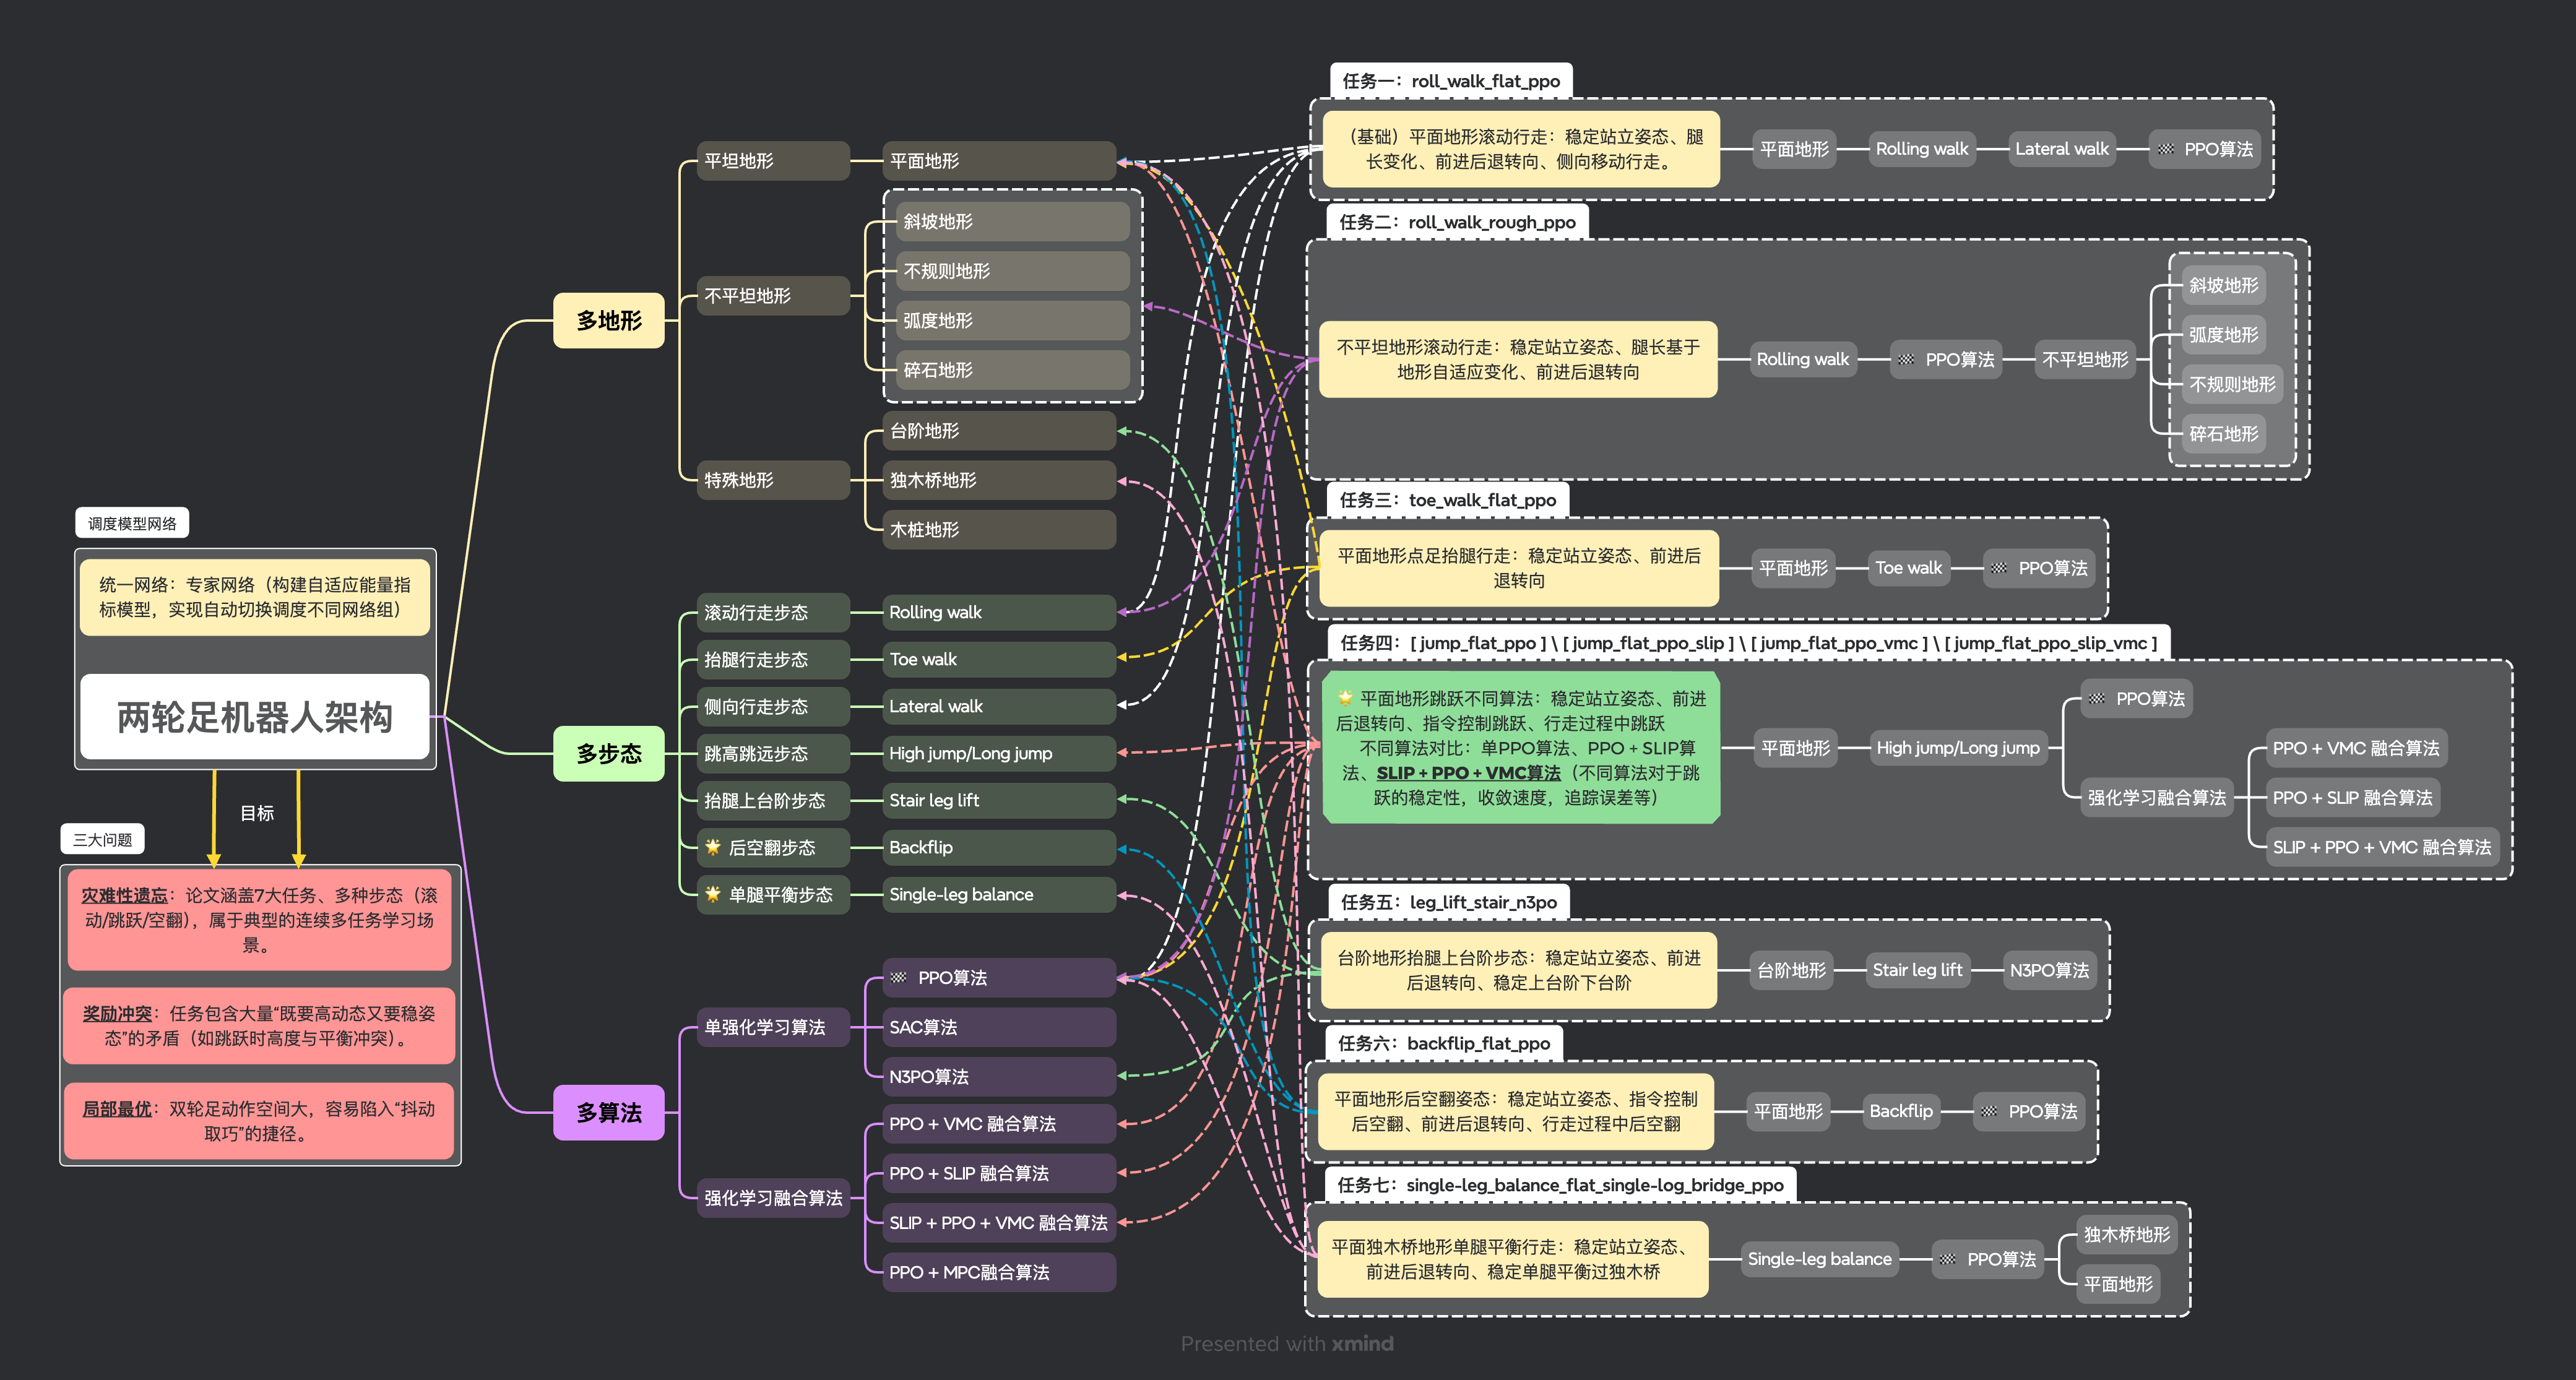
\includegraphics[width=0.98\textwidth]{两轮足机器人架构.png}
    \bicaption{两轮足机器人总体研究架构（多地形-多步态-多算法）}{Overall research architecture of the two-wheeled legged robot (multi-terrain, multi-gait, multi-algorithm)}
    \label{fig:architecture}
\end{figure}

\section{论文组织结构}

本文共分九章，组织结构如图~\ref{fig:structure}所示。

\begin{figure}[!htbp]
    \centering
    
\includegraphics[width=0.95\textwidth]{WUST-flash.pdf}
    \bicaption{论文组织结构图（替换为自绘图）}{Thesis organization structure (replace with your own figure)}
    \label{fig:structure}
\end{figure}

第1章为绪论，阐述研究背景、国内外研究现状与主要研究内容；第2章介绍两轮足机器人建模与强化学习理论基础；第3章设计"分训-整合"的多任务强化学习总体框架与混合地形统一环境；第4-6章分别阐述行走类、精细平衡类与高动态敏捷类步态专家的独立训练；第7章设计学习式统一调度器；第8章进行统一系统集成与整体验证；第9章为结论与展望。

%%% Local Variables:
%%% mode: latex
%%% TeX-master: "../main"
%%% End:

\chapter[两轮足机器人建模与强化学习理论基础]{两轮足机器人建模与强化学习理论基础}
\label{cha:theory}

本章首先建立两轮足机器人的机构、运动学与简化动力学模型，然后介绍强化学习的基础理论框架与本文使用的核心算法（PPO、SAC、N3PO），最后介绍物理仿真平台与异构训练框架，为后续章节的步态控制研究奠定理论与工具基础。

\section{两轮足机器人机构与运动学模型}

\subsection{机构构型与自由度分析}

本文研究的两轮足机器人由基座机身、两条对称分布的腿部机构与两个主动驱动轮组成。每条腿包含髋俯仰、髋横滚、膝俯仰等关节，驱动轮集成于腿末端，具备独立的滚动与转向驱动。机器人整体呈现"轮-腿混合"构型：在平坦地形上以双轮支撑滚动行走，在复杂地形上通过腿部抬升、侧倾实现越障与姿态调节。

以两条腿共$n_l$个旋转关节加上双轮驱动计，机器人总自由度数$n_q = n_l + 2$。机身位姿可用六维广义坐标$\boldsymbol{q}_b \in \mathbb{R}^6$描述，关节角与轮角构成关节坐标$\boldsymbol{q}_j \in \mathbb{R}^{n_q}$，系统的完整广义坐标记为
\begin{equation}
  \boldsymbol{q} = \left[\boldsymbol{q}_b^{\mathrm{T}},\ \boldsymbol{q}_j^{\mathrm{T}}\right]^{\mathrm{T}} \in \mathbb{R}^{6+n_q}.
  \label{eq:qcoord}
\end{equation}

\subsection{运动学建模}

正运动学描述从关节空间到末端（轮心）笛卡尔空间的映射。令$\boldsymbol{T}_{base}^{i}$为第$i$条腿末端的齐次变换矩阵，其由基座位姿与各关节旋转变换连乘得到
\begin{equation}
  \boldsymbol{T}_{base}^{i} = \boldsymbol{T}_{base}^{0}\,\boldsymbol{T}_{0}^{1}\cdots \boldsymbol{T}_{i-1}^{i},
  \label{eq:fk}
\end{equation}
其中$\boldsymbol{T}_{j-1}^{j}$为相邻连杆间的齐次变换。逆运动学则在已知期望轮心位置与姿态的条件下求解关节角$\boldsymbol{q}_j$，本文在步态轨迹规划中采用解析逆解与数值迭代相结合的求解方式。

\subsection{倒立摆动力学模型}

两轮足机器人稳定站立可抽象为车轮-机身的倒立摆模型。以机身倾角$\theta$、车轮角$\phi$与轮轴前进位移$x$为广义坐标，忽略腿部关节动态，系统的简化动力学方程为
\begin{equation}
  \left\{
    \begin{aligned}
      (m_l r^2 + m_w r^2 + m_l d^2\cos\theta)\,\ddot{\theta} &\;=\; m_l g d \sin\theta - \tau_w - m_l d \ddot{x} \cos\theta, \\
      (m_w + m_l)\,\ddot{x} + m_l d\,\ddot{\theta}\cos\theta &\;=\; \tau_w / r + f_{ext},
    \end{aligned}
  \right.
  \label{eq:inverted-pendulum}
\end{equation}
式中，$m_w$为车轮质量，$m_l$为机身等效质量，$d$为机身质心到轮轴的高度，$r$为车轮半径，$g$为重力加速度，$\tau_w$为轮端驱动力矩，$f_{ext}$为外部扰动力。由式~\eqref{eq:inverted-pendulum}可见，系统是典型的欠驱动不稳定系统，其稳定控制依赖轮端力矩的实时反馈调节，这也正是本文采用强化学习学习的核心控制对象。

此外，在跳跃等高动态运动中，本文引入弹簧负载倒立摆（SLIP）模型作为弹道运动的先验模板\cite{blickhan1989,geyer2006}。SLIP模型将机器人的质心运动等效为带弹簧腿的点质量，其着地-离地相的地面反力控制为跳跃轨迹规划提供了简化解析解。

\section{强化学习基础理论}

\subsection{马尔可夫决策过程}

强化学习问题可建模为马尔可夫决策过程（Markov Decision Process, MDP），用五元组$\left(\mathcal{S},\mathcal{A},\mathcal{P},\mathcal{R},\gamma\right)$描述，其中$\mathcal{S}$为状态空间，$\mathcal{A}$为动作空间，$\mathcal{P}(s'|s,a)$为状态转移概率，$\mathcal{R}(s,a)$为奖励函数，$\gamma\in(0,1]$为折扣因子\cite{sutton1998}。策略$\pi(a|s)$给出状态$s$下选择动作$a$的概率，智能体的目标是最大化累计折扣回报
\begin{equation}
  J(\pi) = \mathbb{E}_{\tau \sim \pi}\left[\sum_{t=0}^{\infty}\gamma^t\,r_t\right],
  \label{eq:mdp-objective}
\end{equation}
式中，$\tau = (s_0,a_0,s_1,a_1,\ldots)$为轨迹。

\subsection{策略梯度与PPO算法}

策略梯度方法通过直接对策略参数求梯度以最大化目标函数\eqref{eq:mdp-objective}，其梯度估计为
\begin{equation}
  \nabla_\theta J(\theta) = \mathbb{E}_{s,a\sim\pi_\theta}\left[\nabla_\theta \log\pi_\theta(a|s)\,A^{\pi_\theta}(s,a)\right],
  \label{eq:pg}
\end{equation}
式中，$A^{\pi}(s,a)$为优势函数。近端策略优化（Proximal Policy Optimization, PPO）\cite{ppo2017}在策略梯度中引入裁剪项以限制单步更新幅度，其裁剪目标函数为
\begin{equation}
  L^{CLIP}(\theta) = \mathbb{E}_t\left[\min\left(r_t(\theta)\hat{A}_t,\ \operatorname{clip}\left(r_t(\theta),1-\varepsilon,1+\varepsilon\right)\hat{A}_t\right)\right],
  \label{eq:ppo-clip}
\end{equation}
式中，$r_t(\theta) = \pi_\theta(a_t|s_t)/\pi_{\theta_{old}}(a_t|s_t)$为新旧策略的概率比，$\varepsilon$为裁剪系数。裁剪项使得策略更新不会过度偏离旧策略，保证了训练的稳定性，是本文各步态任务的基础算法。

\subsection{最大熵强化学习与SAC算法}

软演员-评论家（Soft Actor-Critic, SAC）\cite{sac2018}在目标中引入策略熵最大化，鼓励探索并提升策略的随机鲁棒性，其目标函数为
\begin{equation}
  J(\pi) = \mathbb{E}_{s,a\sim\pi}\left[\sum_{t}\gamma^t\left(r_t + \alpha\,\mathcal{H}\left(\pi(\cdot|s_t)\right)\right)\right],
  \label{eq:sac-objective}
\end{equation}
式中，$\alpha$为温度系数，$\mathcal{H}(\cdot)$为策略熵。SAC属于离策略（off-policy）算法，样本效率较高，本文将其作为抬腿上台阶等精细任务的对比算法之一。

\subsection{约束马尔可夫决策过程与N3PO}

当任务同时包含性能指标与安全性约束时，问题可建模为约束马尔可夫决策过程（CMDP）。在CMDP中，除原始回报外还引入代价函数$c(s,a)$，策略优化问题表述为
\begin{equation}
  \begin{aligned}
    \max_{\pi}\;&\mathbb{E}_{\tau\sim\pi}\left[\sum_{t}\gamma^t r_t\right]\\
    \text{s.t.}\;&\mathbb{E}_{\tau\sim\pi}\left[\sum_{t}\gamma^t c_t\right] \le d,
  \end{aligned}
  \label{eq:cmdp}
\end{equation}
式中，$d$为代价预算上限。N3PO（Natural Policy Gradient with safety constraints）算法基于自然策略梯度\cite{npg2001}与约束投影\cite{cpo2017}，在每次策略更新中显式满足约束，适用于"既要高动态又要稳姿态"的精细控制任务。本文在抬腿上台阶任务中引入N3PO，约束项包括关节力矩饱和率、机身姿态范围与轮端净空等。

\subsection{分层强化学习与门控机制}

当任务可分解为"高层决策 + 底层执行"两个层次时，可采用分层强化学习（Hierarchical Reinforcement Learning, HRL）框架。选项（Option）框架\cite{sutton1999}将高层决策抽象为选项集合，每个选项包含一条底层策略及其终止条件，高层策略负责在选项之间进行选择。在机器人运动控制中，底层选项即各步态专家策略，高层策略即统一调度器，二者的双层结构天然契合本文"分训-整合"的总体思路。

专家混合（Mixture of Experts, MoE）\cite{jacobs1991,shazeer2017}通过门控网络对多个专家网络的输出进行加权组合，实现对不同能力的按需激活。在调度器中，门控网络接收地形感知与本体状态，输出对各步态专家的选择权重，既可采用硬门控（仅激活最高权重专家，响应快、便于工程部署），也可采用软门控（各专家输出加权混合，切换平滑），还可通过嵌入空间技能抽象\cite{hausman2018}或多样性技能学习\cite{eysenbach2019}学习可迁移的高层表征。本文第7章的学习式统一调度器即基于上述分层强化学习与门控机制设计。

\section{物理仿真与异构训练框架}

\subsection{MuJoCo物理引擎}

MuJoCo（Multi-Joint dynamics with Contact）是一款高效、稳定的多体接触动力学仿真引擎\cite{todorov2012}，以其快速而精确的接触求解、良好的可微性而被广泛用于机器人控制研究。本文基于MuJoCo搭建两轮足机器人的仿真环境，包括机构模型定义、地形场景构建（平面、斜坡、碎石、台阶、独木桥、木桩等）、观测与奖励接口封装以及领域随机化模块。

\subsection{UniLab异构强化学习训练框架}

面向两轮足机器人多步态训练需求，本文采用自主研发的UniLab异构强化学习框架，其核心思想是将CPU上的多线程物理仿真与GPU/加速器上的策略训练解耦，通过统一共享内存的循环缓冲区（Shared Replay Buffer）传输transition，从而实现大规模并行仿真下的高效训练。该框架统一了PPO、SAC等算法的训练接口，支持"配置即任务"的Hydra配置体系，能够通过修改任务配置文件快速切换地形、奖励与算法，是本文四大模块、七大任务统一训练与对比验证的工程基础。

\section{本章小结}

本章建立了两轮足机器人的机构、运动学与倒立摆动力学模型，阐明了其欠驱动不稳定的控制本质；介绍了MDP框架、PPO、SAC与N3PO等强化学习核心算法及CMDP约束优化思想；引入了分层强化学习与门控机制，为学习式统一调度器的设计奠定理论基础；并介绍了MuJoCo物理引擎与UniLab异构训练框架。上述模型、算法与工具共同构成后续章节多步态运动控制研究的理论基础。

%%% Local Variables:
%%% mode: latex
%%% TeX-master: "../main"
%%% End:

\chapter[多任务强化学习总体框架与混合地形统一环境]{多任务强化学习总体框架与混合地形统一环境}
\label{cha:framework}

本章针对两轮足机器人"多地形、多步态、多算法"的综合任务需求，提出"分训-整合"两阶段的多任务强化学习总体框架：第一阶段分别训练7个步态专家策略，第二阶段以学习式统一调度器将各专家整合至混合地形统一环境中，实现按地形自适应切换步态。本章首先给出总体设计思路，然后阐述混合地形统一环境设计、步态专家库划分与学习式调度器的总体方案，最后说明三大核心问题（灾难性遗忘、奖励冲突、局部最优）的应对策略。

\section{总体设计思路}

\subsection{设计需求分析}

综合前文分析，总体框架需要满足以下设计需求：

（1）\textbf{多步态覆盖}：支持滚动行走、侧向移动、粗糙地形行走、抬腿行走、跳跃、后空翻、抬腿上台阶与单腿平衡等步态能力；

（2）\textbf{多地形适应}：覆盖平面、粗糙、碎石、斜坡、台阶、弧度、独木桥、木桩与狭窄通道等多种地形，并能在混合地形环境中自动切换步态；

（3）\textbf{多算法融合}：支持单PPO、PPO+SLIP、SLIP+PPO+VMC、N3PO等算法范式的统一接入与对比；

（4）\textbf{多任务整合}：系统性地缓解灾难性遗忘、奖励冲突与局部最优三大问题。

\subsection{"分训-整合"两阶段范式}

针对单一策略难以同时掌握多种步态、直接统一训练又易遗忘与冲突的难题，本文提出"分训-整合"两阶段范式，如图~\ref{fig:paradigm}所示。

\textbf{第一阶段（分训）}：将综合任务分解为7类典型步态子任务，每类步态在对应地形的专用环境中独立训练，得到7个参数解耦的步态专家策略网络。各专家互不干扰，训练目标单一明确，从根本上规避了多任务共同训练导致的灾难性遗忘与奖励冲突。

\textbf{第二阶段（整合）}：将7个步态专家作为底层选项集合，设计学习式统一调度器。调度器在混合地形统一环境中训练，学习依据地形感知与本体状态自动选择或混合激活合适的步态专家，实现机器人从起点到终点的完整遍历与按地形自适应步态切换。

\begin{figure}[!htbp]
    \centering
    
\includegraphics[width=0.95\textwidth]{WUST-flash.pdf}
    \bicaption{"分训-整合"两阶段范式示意图（替换为自绘架构图）}{Schematic of the two-phase "train-then-integrate" paradigm (replace with your own figure)}
    \label{fig:paradigm}
\end{figure}

\section{混合地形统一仿真环境设计}

\subsection{地形库构成}

为验证多步态整合与按地形自动切换效果，本文构建包含多种地形单元的混合地形统一仿真环境，地形库如表~\ref{tab:terrain-lib}所示。

\begin{table}[!htbp]
    \centering
    \bicaption{混合地形统一环境的地形库构成}{Terrain library of the unified mixed-terrain environment}
    \resizebox{0.95\textwidth}{!}{
        \begin{tabular}{clp{5.6cm}}
            \toprule[1.5pt]
            地形单元 & 关键特征 & 设计目的 \\
            \midrule[0.75pt]
            平面地形 & 平整连续 & 滚动行走、侧向移动基础验证 \\
            粗糙/碎石地形 & 高度起伏、接触随机 & 验证抬腿点足与粗糙行走专家 \\
            斜坡地形 & 坡角变化 & 验证地形自适应腿长调节 \\
            台阶地形（低/高） & 不同台阶高度 & 低阶抬腿跨越、高阶跳跃上去 \\
            独木桥地形 & 窄支撑面 & 验证单腿平衡专家 \\
            木桩/间隙地形 & 离散支撑、有间隙 & 验证跳跃专家跨越间隙 \\
            狭窄通道 & 转向空间受限 & 验证侧向移动专家 \\
            \bottomrule[1.5pt]
        \end{tabular}
    }
    \label{tab:terrain-lib}
\end{table}

\subsection{地形-步态对应关系}

按地形自动切换步态是整合阶段的核心目标，本文明确各典型地形与最适步态专家的对应关系，作为调度器训练的期望行为与验收基准，如表~\ref{tab:terrain-gait}所示。

\begin{table}[!htbp]
    \centering
    \bicaption{典型地形与最适步态的对应关系}{Correspondence between typical terrains and preferred gaits}
    \resizebox{0.95\textwidth}{!}{
        \begin{tabular}{lcp{4.6cm}}
            \toprule[1.5pt]
            地形场景 & 采用步态 & 理由 \\
            \midrule[0.75pt]
            粗糙/碎石地形 & 抬腿点足行走 & 减少轮端颠簸、提高越障能力 \\
            低台阶地形 & 抬腿跨越 & 小位移精细跨越，稳定高效 \\
            高台阶地形 & 跳跃上去 & 超出抬腿范围，需要弹道起跳 \\
            狭窄通道地形 & 侧向移动 & 横向位移，避免大半径转向 \\
            独木桥地形 & 单腿平衡 & 缩小有效支撑宽度，精确过桥 \\
            木桩/间隙地形 & 跳跃通过 & 跨越支撑间隙 \\
            平坦开阔地形 & 滚动行走 & 高效平稳 \\
            \bottomrule[1.5pt]
        \end{tabular}
    }
    \label{tab:terrain-gait}
\end{table}

\subsection{领域随机化}

为提升策略与调度器的鲁棒性、抑制局部最优，统一环境在训练中随机化机器人质量、质心位置、摩擦系数、地形参数（坡角、台阶高度、间隙宽度）等物理量，并施加随机外部扰动力，迫使策略与调度器学习不依赖特定参数的鲁棒控制与决策方式\cite{tobin2017,peng2018}。

\section{步态专家库的独立训练}

\subsection{7个步态专家的划分}

依据综合任务需求，本文将步态能力划分为7个步态专家，如表~\ref{tab:experts}所示。每个专家对应一个独立的策略网络，在对应地形的专用环境中训练。

\begin{table}[!htbp]
    \centering
    \bicaption{步态专家库划分与训练配置}{Gait expert library and training configuration}
    \resizebox{0.95\textwidth}{!}{
        \begin{tabular}{clll}
            \toprule[1.5pt]
            序号 & 步态专家 & 适用地形 & 训练算法 \\
            \midrule[0.75pt]
            1 & 滚动行走专家（含侧向移动） & 平面、狭窄通道 & PPO \\
            2 & 粗糙地形行走专家 & 粗糙、碎石、斜坡 & PPO \\
            3 & 抬腿行走专家 & 粗糙、木桩 & PPO \\
            4 & 跳跃专家 & 高台阶、间隙 & PPO / PPO+SLIP / SLIP+PPO+VMC \\
            5 & 后空翻专家 & 平面（特殊动作） & PPO（确定性翻转） \\
            6 & 抬腿上台阶专家 & 台阶（低） & N3PO \\
            7 & 单腿平衡专家 & 独木桥、狭窄 & PPO \\
            \bottomrule[1.5pt]
        \end{tabular}
    }
    \label{tab:experts}
\end{table}

\subsection{专家独立训练与验收}

各步态专家采用统一的观测组织方式（本体状态 + 地形感知 + 任务指令）与训练流程，在专用环境中训练至各自验收标准（如站立时长、速度跟踪误差、成功率等）。由于各专家参数完全解耦，独立训练过程互不影响，从结构上规避了多步态连续学习带来的灾难性遗忘。第4-6章将分别阐述行走类、精细平衡类与高动态敏捷类专家的具体训练细节。

\subsection{观测、动作与执行频率设计}

观测空间按"本体状态 + 地形感知 + 任务指令"三部分组织，各专家依据任务特点动态扩展维度（如跳跃专家追加起跳标志与飞行阶段信息，单腿平衡专家追加FSM状态与轮地接触历史）。动作空间定义为各关节目标角与轮端目标速度（或力矩）。基础行走类专家采用100Hz控制率，高动态专家（跳跃、后空翻）采用200Hz控制率，热启动迁移时保持控制率对齐。

\section{学习式统一调度器总体方案}

\subsection{调度器任务建模}

统一调度器将"按地形选择步态"建模为分层强化学习问题：底层为7个步态专家构成的选项集合，高层为调度策略$\pi_h$。调度器在时刻$t$接收地形感知特征$\boldsymbol{\phi}_t$与本体状态$\boldsymbol{s}_t$，输出对专家$i$的选择概率
\begin{equation}
  \pi_h(i\,|\,\boldsymbol{\phi}_t,\boldsymbol{s}_t) = \frac{\exp\left(f_i(\boldsymbol{\phi}_t,\boldsymbol{s}_t)/\tau\right)}{\sum_{j=1}^{M}\exp\left(f_j(\boldsymbol{\phi}_t,\boldsymbol{s}_t)/\tau\right)},
  \label{eq:scheduler}
\end{equation}
式中，$f_i(\cdot)$为调度网络对专家$i$的得分，$M$为专家数量，$\tau$为温度系数。调度器可采用硬门控（激活得分最高的专家）或软门控（按概率加权混合专家动作）。

\subsection{调度器训练}

调度器在混合地形统一环境中训练，其高层奖励综合任务完成度、遍历速度与稳定性等指标。训练采用课程式场景编排：由单地形单元逐步过渡到多地形交替，最终在完整混合地形环境中训练，使调度器逐步学会"地形感知-步态选择"的映射关系。调度器训练过程中，各步态专家可保持冻结以验证调度本身的有效性，也可在后期进行联合微调以进一步提升整体性能。

\subsection{与三大问题的关系}

"分训-整合"范式与三大核心问题的关系如下：各专家参数解耦避免了灾难性遗忘；各专家独立奖励与调度器高层目标分离缓解了奖励冲突；混合地形统一环境的细粒度评估与领域随机化抑制了局部最优。具体机制在第3.5节详细阐述。

\section{多任务整合的三大核心问题应对}

\subsection{灾难性遗忘：参数解耦与分训}

传统的单一网络按序学习多步态时，新步态的参数更新会覆盖旧步态知识，导致灾难性遗忘\cite{mccloskey1989,kirkpatrick2017}。本文通过"分训-整合"范式从结构上化解该问题：7个步态专家各自拥有独立的网络参数，分训阶段互不干扰；整合阶段调度器仅在专家之间进行选择，不直接修改专家参数（除非联合微调），因此任何步态能力的习得都不会破坏其他步态能力。

\subsection{奖励冲突：专家奖励与调度器目标分离}

多步态任务中"跳得高""走得稳""姿态受限"等子目标相互矛盾，若合并为单一奖励函数将难以优化。本文将该冲突通过分层结构分离：每个专家在各自的专用环境中拥有专属的、内部自洽的奖励函数（如跳跃专家专注跳跃高度与落地稳定）；调度器拥有独立的高层目标（如遍历完成度），不直接叠加专家内部奖励。通过"底层各管各的目标、高层只管选谁干"，奖励冲突被结构性消解。

\subsection{局部最优：统一评估与领域随机化}

为规避策略"抖动取巧"等局部最优，本文一方面建立统一的细粒度评估指标体系（平移/航向跟踪误差、成功率、轮端净空、落地冲击、关节力矩饱和度等），从多维度揭示策略行为是否走捷径；另一方面通过强领域随机化迫使策略学习鲁棒控制而非依赖特定参数的模式。

\section{多维评价与分析体系}

本文建立贯穿分训与整合两个阶段的统一评价体系：分训阶段评估各专家的步态性能与算法对比指标；整合阶段评估调度器在混合地形环境中的遍历成功率、步态切换次数、切换过程姿态扰动以及各地形段落的通过情况，并以多维度雷达图与统计表形式呈现。三大问题的消融验证（去调度直接统一训练、去领域随机化等）也基于该评价体系开展。

\section{本章小结}

本章提出"分训-整合"两阶段的多任务强化学习总体框架，设计了混合地形统一仿真环境与地形-步态对应关系，划分了7个步态专家并阐述其独立训练方案，给出了学习式统一调度器的总体建模与训练思路，并从参数解耦、奖励分离、统一评估三个层面阐述了三大核心问题的应对策略。后续第4-6章阐述步态专家训练细节，第7章阐述调度器设计，第8章进行统一系统集成与整体验证。

%%% Local Variables:
%%% mode: latex
%%% TeX-master: "../main"
%%% End:

\chapter[行走类步态专家的独立训练]{行走类步态专家的独立训练}
\label{cha:walking-experts}

本章对应"分训"阶段的第一类专家——行走类步态专家，阐述滚动行走专家（含侧向移动）与粗糙地形行走专家两个专家网络的独立训练。两者分别覆盖平面/狭窄地形与粗糙/碎石/斜坡地形的行走能力，是调度器在开阔与中等复杂度地形上的基础选项。

\section{行走类专家库概述}

行走类专家库包含两个专家：

（1）\textbf{滚动行走专家}：面向平面与狭窄通道地形，实现稳定站立、前进后退、转向与侧向移动等基础能力，控制频率100Hz，采用PPO算法训练；

（2）\textbf{粗糙地形行走专家}：面向粗糙、碎石、斜坡等地形，实现基于地形感知的腿长自适应变化与鲁棒行走，同样采用PPO算法训练。

两类专家共用统一的观测组织方式与训练流程，但因适用地形与能力侧重不同，观测维度与奖励结构存在差异，故独立训练、独立验收。

\section{滚动行走专家}

\subsection{稳定站立姿态控制}

稳定站立是滚动行走专家的首要控制目标。基于第2章的倒立摆模型，策略需要输出轮端力矩以实时抑制机身倾角发散。奖励函数中基础平衡项设计为
\begin{equation}
  r_{bal} = \exp\left(-\lambda_1\,\theta_{pitch}^2 - \lambda_2\,\omega_{pitch}^2\right),
  \label{eq:rbal}
\end{equation}
式中，$\theta_{pitch}$为机身俯仰角，$\omega_{pitch}$为其角速度，$\lambda_1$、$\lambda_2$为权重。同时引入姿态角速度惩罚与动作平滑惩罚，防止剧烈晃动，规避"抖动取巧"的局部最优。

\subsection{腿长变化与行走机制}

滚动行走通过腿部关节的协同伸缩改变机身质心高度与轮端支撑构型。本文在动作空间中显式包含腿部关节目标角，并引入腿长相关的奖励项约束质心高度
\begin{equation}
  r_{leg} = \exp\left(-\lambda_3\,(h_{com} - h_{ref})^2\right),
  \label{eq:rleg}
\end{equation}
式中，$h_{com}$为质心高度，$h_{ref}$为参考质心高度。通过腿长变化调节，机器人能够实现低重心稳定行走与姿态过渡。

\subsection{前进后退与转向控制}

前进后退通过跟踪线速度指令实现，转向通过跟踪偏航角速度指令实现。速度跟踪奖励定义为
\begin{equation}
  r_{vel} = \exp\left(-\lambda_4\,\|\boldsymbol{v}_t - \boldsymbol{v}_{cmd}\|^2\right),
  \label{eq:rvel}
\end{equation}
式中，$\boldsymbol{v}_t$为实际速度，$\boldsymbol{v}_{cmd}$为指令速度。训练中采用课程式速度调度，将指令速度由低速逐步提升至高速。

\subsection{侧向移动（狭窄地形）}

在滚动行走基础上，本文进一步训练侧向移动能力，使机器人能够在保持航向的同时沿横向移动。该能力在狭窄通道等转向空间受限的场景中尤为重要——调度器可据此选择"侧向移动"而非"大半径转向"通过狭窄地形。侧向移动通过在奖励中增加横向速度跟踪项实现，其运动学由轮端差速驱动与腿部侧倾配合完成。

\section{粗糙地形行走专家}

\subsection{地形感知与观测设计}

为实现地形自适应，粗糙地形行走专家在观测空间中引入地形感知信息，包括前向地面高度剖面与轮地接触状态。定义地形高度剖面为
\begin{equation}
  \boldsymbol{h}_{terr} = \left[h_{-N}, \ldots, h_0, \ldots, h_{N}\right]^{\mathrm{T}},
  \label{eq:terrain-probe}
\end{equation}
式中，$h_i$为机器人前方第$i$个采样点的地面相对高度。观测空间由"本体状态 + 地形高度剖面 + 任务指令"构成，策略据此提前感知地形变化并规划腿长与姿态。

\subsection{腿长基于地形自适应变化}

策略依据地形高度剖面实时调整腿长，使轮端保持有效接触并维持机身水平。定义腿长补偿量为
\begin{equation}
  \Delta L = K_p\,(h_{ref} - \hat{h}_{front}) + K_d\,(\dot{h}_{ref} - \dot{\hat{h}}_{front}),
  \label{eq:leg-adapt}
\end{equation}
式中，$\hat{h}_{front}$为前方地形估计高度，$h_{ref}$为参考高度，$K_p$、$K_d$为增益。该补偿量作为任务指令输入策略，作为腿长控制的先验引导。

\subsection{多地形课程训练}

粗糙地形行走专家采用"多地形混合 + 逐地形课程"的训练策略：先在平面地形上热启动，再逐步引入斜坡、碎石等单一地形，最后进行多地形混合训练。各典型地形的训练要点如下：

\textbf{斜坡地形}：侧重姿态稳定与坡面适应，奖励中增加机身俯仰角与坡角匹配项，避免下坡失控。

\textbf{碎石地形}：碎石地面接触点随机变化，侧重轮地接触鲁棒性与速度跟踪平滑性，强化领域随机化以提升对随机接触扰动的适应能力。

\section{行走类专家独立训练实验设置}

实验基于MuJoCo物理引擎与UniLab异构训练框架，行走类专家的公共训练参数如表~\ref{tab:setup-walk}所示。

\begin{table}[!htbp]
    \centering
    \bicaption{行走类专家训练实验设置}{Experiment setup for walking expert training}
    \resizebox{0.92\textwidth}{!}{
        \begin{tabular}{lcl}
            \toprule[1.5pt]
            参数 & 数值 & 说明 \\
            \midrule[0.75pt]
            控制频率 & 100Hz & 策略推理频率 \\
            算法 & PPO & 近端策略优化 \\
            折扣因子 & 0.99 & $\gamma$ \\
            裁剪系数 & 0.2 & $\varepsilon$ \\
            训练地形 & 平面/粗糙/碎石/斜坡 & 分专家设置 \\
            随机种子数 & 5 & 评估稳定性 \\
            \bottomrule[1.5pt]
        \end{tabular}
    }
    \label{tab:setup-walk}
\end{table}

\section{实验结果与分析}

\subsection{滚动行走专家性能}

【待填入：滚动行走速度跟踪误差、航向误差、站立稳定时间、侧向移动精度等实验结果，并附训练曲线图与步态截图。】

\subsection{粗糙地形行走专家性能}

【待填入：各粗糙地形通过率、速度跟踪误差、姿态角标准差（参照表~\ref{tab:terrain-result}结构），以及不同领域随机化强度下的鲁棒性对比。】

\begin{table}[!htbp]
    \centering
    \bicaption{粗糙地形行走实验结果（示意表格，填入真实数据）}{Rough-terrain walking results (illustrative, fill in real data)}
    \resizebox{0.92\textwidth}{!}{
        \begin{tabular}{lccc}
            \toprule[1.5pt]
            地形类型 & 通过率(\%) & 速度跟踪误差(m/s) & 姿态角标准差($^\circ$) \\
            \midrule[0.75pt]
            斜坡（$10^\circ$） & 【待填】 & 【待填】 & 【待填】 \\
            碎石地形 & 【待填】 & 【待填】 & 【待填】 \\
            粗糙地形 & 【待填】 & 【待填】 & 【待填】 \\
            \bottomrule[1.5pt]
        \end{tabular}
    }
    \label{tab:terrain-result}
\end{table}

\section{本章小结}

本章阐述了行走类步态专家（滚动行走专家与粗糙地形行走专家）的独立训练方法。滚动行走专家实现了稳定站立、腿长变化、前进后退、转向与侧向移动等基础能力；粗糙地形行走专家通过地形感知观测设计、腿长自适应补偿与多地形课程训练，实现了粗糙、碎石、斜坡等非结构化地形上的稳定行走。两类专家作为调度器的底层基础选项，为第8章统一系统集成提供了行走能力支撑。

%%% Local Variables:
%%% mode: latex
%%% TeX-master: "../main"
%%% End:

\chapter[精细平衡类步态专家的独立训练]{精细平衡类步态专家的独立训练}
\label{cha:fine-experts}

本章对应"分训"阶段的第二类专家——精细平衡类步态专家，阐述抬腿行走专家、抬腿上台阶专家与单腿平衡专家三个专家网络的独立训练。三者均要求在大范围抬腿/重心转移的同时保持姿态稳定，涉及"高动态动作"与"精细平衡"的矛盾，是精细控制与约束强化学习的典型应用。

\section{精细平衡类专家库概述}

精细平衡类专家库包含三个专家：

（1）\textbf{抬腿行走专家}：面向粗糙与木桩地形，通过周期抬腿实现"点足"行走，为越障与精细化操控提供步态基础，采用PPO训练；

（2）\textbf{抬腿上台阶专家}：面向低台阶地形，实现稳定抬腿跨越台阶，采用N3PO约束强化学习训练；

（3）\textbf{单腿平衡专家}：面向独木桥与狭窄地形，实现单侧轮支撑平衡行走，采用PPO训练。

该类任务的共同难点在于约束苛刻且动作与稳定目标冲突剧烈，若不显式处理约束，策略极易在"抬腿高度"与"平衡保持"之间顾此失彼，或陷入剧烈晃动的局部最优。

\section{抬腿行走专家}

\subsection{抬腿机制与任务设计}

抬腿行走通过周期性地抬起单侧腿、以另一侧轮/腿支撑实现"点足"行走。其观测空间在基础观测上追加腿部抬升高度、相位计时器与轮地接触标志等维度。任务定义与滚动行走类似，但以"抬腿高度跟踪"与"支撑稳定性"作为核心奖励项。

\subsection{粗糙与木桩地形的点足行走}

在粗糙地形上，滚动行走轮端颠簸明显、越障能力有限，而抬腿点足行走能够主动选择支撑点、减小轮端无效接触。在木桩地形上，机器人需在有限离散支撑点之间规划落脚位置。因此，本文将该专家设计为调度器在粗糙与木桩地形的首选选项——这也是第3章表~\ref{tab:terrain-gait}中"粗糙/碎石地形→抬腿点足行走"对应关系的实现基础。

\section{抬腿上台阶专家}

\subsection{任务定义与约束分析}

抬腿上台阶要求机器人在保持稳定站立与前进后退转向能力的前提下，将单侧腿抬起并跨越台阶边缘，完成上台阶与下台阶动作。任务的关键约束包括：关节力矩饱和限制、轮端净空要求、机身姿态范围限制以及落地冲击限制。

\subsection{基于N3PO的约束强化学习}

本章将上台阶任务建模为约束马尔可夫决策过程（CMDP）。在总奖励中保留基础能力奖励项的同时，将关键安全指标建模为代价函数并纳入N3PO的约束优化框架
\begin{equation}
  \begin{aligned}
    \max_{\pi}\;&\mathbb{E}\left[\sum_t \gamma^t\left(r_{task} + w\,r_{base}\right)\right],\\
    \text{s.t.}\;&\mathbb{E}\left[\sum_t \gamma^t\, c_{sat}\right] \le d_1,\quad
    \mathbb{E}\left[\sum_t \gamma^t\, c_{tilt}\right] \le d_2,
  \end{aligned}
  \label{eq:n3po-cmdp}
\end{equation}
式中，$c_{sat}$为关节力矩饱和度代价，$c_{tilt}$为机身倾角越界代价，$d_1$、$d_2$为对应预算。N3PO基于自然策略梯度在每次更新中显式满足约束，保证策略在优化抬腿性能的同时不突破安全边界。

\subsection{与SAC及单强化学习算法的对比}

为验证N3PO的有效性，本章在同一上台阶任务上实现SAC算法与单强化学习算法（纯PPO）作为对比基线。对比指标包括上/下台阶成功率、力矩饱和度、姿态越界率与训练收敛速度，重点考察约束强化学习在"高动态 + 强约束"场景下的优势。

\section{单腿平衡专家}

\subsection{收膝折腿与侧倾机制}

单腿平衡指机器人将重心完全转移至单侧支撑轮，另一侧轮抬离地面，从而获得更窄的等效支撑宽度。为降低支撑难度，本文采用\textbf{收膝折腿}机制：支撑腿收膝下蹲降低质心高度，抬离腿收膝折叠，同时机身向支撑侧侧倾（约$28^\circ$），使质心投影落入支撑轮接触区域内。

与后空翻的"弹道可开环"不同，单腿平衡的保持本质上是倒立摆调节，必须闭环控制。因此，前馈（FF）仅用于折腿与落腿的过渡阶段，横滚平衡等核心调节完全交由强化学习策略闭环实现，其横滚角奖励定义为
\begin{equation}
  r_{roll} = \exp\left(-\lambda\,\left(\frac{up\_y - \cos\theta_{ref}}{\cos\theta_{ref}}\right)^2\right),
  \label{eq:rroll}
\end{equation}
式中，$up\_y$为机身法向在世界系$y$方向的分量，$\theta_{ref}$为参考侧倾角。该奖励在直立时接近0、达到参考侧倾时接近1，引导策略平滑学习侧倾平衡。

\subsection{独木桥行走}

在单腿平衡基础上，本章将步态迁移至单木桥地形：桥面窄、两侧无支撑，机器人需在保持单腿平衡的同时完成前进与转向，对横滚稳定裕度与转向精度要求极高。训练采用热启动方式，将滚动行走专家权重迁移至单腿平衡任务，并通过观测网络输入层扩展（追加FSM状态、计时器与轮地接触历史）适配新任务观测，实现知识迁移与网络扩展。

\section{实验结果与分析}

【待填入：（1）抬腿行走专家在粗糙/木桩地形上的抬腿高度跟踪误差、支撑稳定性、通过率；（2）抬腿上台阶的上/下台阶成功率、力矩饱和度与姿态越界率，N3PO与SAC、单强化学习算法的对比结果；（3）单腿平衡保持时长、横滚角标准差、独木桥通过率与转向精度实验结果，建议以表~\ref{tab:fine-result}汇总对比指标。】

\begin{table}[!htbp]
    \centering
    \bicaption{精细平衡专家对比结果（示意表格，填入真实数据）}{Comparison results of fine balance experts (illustrative, fill in real data)}
    \resizebox{0.92\textwidth}{!}{
        \begin{tabular}{lccc}
            \toprule[1.5pt]
            指标 & N3PO & SAC & 单强化学习 \\
            \midrule[0.75pt]
            上台阶成功率(\%) & 【待填】 & 【待填】 & 【待填】 \\
            力矩饱和度 & 【待填】 & 【待填】 & 【待填】 \\
            单腿平衡时长(s) & 【待填】 & 【待填】 & 【待填】 \\
            独木桥通过率(\%) & 【待填】 & 【待填】 & 【待填】 \\
            \bottomrule[1.5pt]
        \end{tabular}
    }
    \label{tab:fine-result}
\end{table}

\section{本章小结}

本章阐述了精细平衡类步态专家（抬腿行走、抬腿上台阶、单腿平衡）的独立训练方法。抬腿行走专家通过点足抬腿实现粗糙与木桩地形的越障行走；抬腿上台阶专家通过N3PO约束强化学习，在满足力矩与姿态约束的前提下实现稳定上台阶；单腿平衡专家通过收膝折腿与机身侧倾机制，结合热启动迁移实现独木桥行走。三者作为调度器在精细地形场景的专家选项，为统一系统集成提供了精细化操控能力。

%%% Local Variables:
%%% mode: latex
%%% TeX-master: "../main"
%%% End:

\chapter[高动态敏捷类步态专家的独立训练]{高动态敏捷类步态专家的独立训练}
\label{cha:agile-experts}

本章对应"分训"阶段的第三类专家——高动态敏捷类步态专家，阐述跳跃专家与后空翻专家两个专家网络的独立训练。跳跃专家面向高台阶与木桩间隙地形，构建单PPO、PPO+SLIP、SLIP+PPO+VMC三种算法范式并对比；后空翻专家面向特殊动作需求，采用确定性翻转方案训练。二者重点解决"既要高动态又要稳姿态"的奖励冲突问题与高动态动作的收敛稳定性问题。

\section{高动态敏捷类专家库概述}

高动态敏捷类专家库包含两个专家：

（1）\textbf{跳跃专家}：面向高台阶与木桩间隙地形，实现指令控制跳跃（跳高/跳远）及行走过程中的跳跃，训练算法涵盖单PPO、PPO+SLIP、SLIP+PPO+VMC三种范式，控制频率200Hz；

（2）\textbf{后空翻专家}：面向平面地形的特殊动作，实现指令控制后空翻，采用基于有限状态机的确定性翻转方案，控制频率200Hz。

高动态运动的核心难点是\textbf{奖励冲突}：跳跃/空翻需要大幅度的爆发动作，而稳定性要求抑制姿态发散，二者奖励信号相互矛盾。若采用单一奖励函数，策略极易陷入"不敢跳"或"跳后失控"的次优解。为此，本章采用阶段式奖励塑形与融合算法两类手段加以应对。

\section{SLIP模型与VMC融合控制基础}

\subsection{SLIP模型}

弹簧负载倒立摆（Spring-Loaded Inverted Pendulum, SLIP）模型将机器人简化为带无质量弹簧腿的点质量，其质心运动由摆动相与着地相交替构成\cite{blickhan1989,geyer2006}。着地相质心轨迹满足
\begin{equation}
  m\,\ddot{\boldsymbol{p}} = m\boldsymbol{g} + k\,(l_0 - \|\boldsymbol{p} - \boldsymbol{p}_{foot}\|)\,\frac{\boldsymbol{p} - \boldsymbol{p}_{foot}}{\|\boldsymbol{p} - \boldsymbol{p}_{foot}\|},
  \label{eq:slip}
\end{equation}
式中，$m$为等效质量，$\boldsymbol{p}$为质心位置，$\boldsymbol{p}_{foot}$为足端位置，$k$为弹簧刚度，$l_0$为自然腿长。SLIP模型为跳跃的起跳、腾空与落地提供了解析的弹道先验，可用于规划参考质心轨迹或生成前馈动作。

\subsection{虚拟模型控制（VMC）}

虚拟模型控制（Virtual Model Control, VMC）\cite{pratt2001}通过在机器人质心处构造虚拟力/力矩，再经雅可比映射为各关节力矩。设虚拟力为$\boldsymbol{F}_{v}$，则关节力矩为
\begin{equation}
  \boldsymbol{\tau} = \boldsymbol{J}^{\mathrm{T}}\,\boldsymbol{F}_{v},
  \label{eq:vmc}
\end{equation}
式中，$\boldsymbol{J}$为任务空间雅可比矩阵。VMC将"质心运动控制"与"关节执行"解耦，便于叠加平衡约束，本文将其用于落地缓冲与姿态保持的力分配。

\section{跳跃专家}

\subsection{单PPO算法}

$jump\_flat\_ppo$ 采用纯强化学习范式，策略直接由观测映射至关节/轮端动作，所有跳跃阶段行为均由奖励驱动学习。该方法实现简单、不依赖模型，但高维动作空间下收敛慢、易受奖励冲突影响。

\subsection{PPO+SLIP融合算法}

$jump\_flat\_ppo\_slip$ 将SLIP模型的弹道先验引入强化学习：由SLIP规划跳跃参考质心轨迹，PPO策略以轨迹跟踪误差作为奖励反馈学习控制动作。该范式将弹道运动的高层规划交给解析模型，强化学习专注低层跟踪控制，显著降低了奖励冲突与学习难度。

\subsection{SLIP+PPO+VMC融合算法}

$jump\_flat\_ppo\_slip\_vmc$ 进一步引入VMC：SLIP负责规划，VMC负责落地与姿态阶段的力分配与缓冲，PPO负责整体策略学习与任务调度。三种先验的融合使各阶段"各司其职"——起跳由SLIP规划主导、空中由策略调节、落地由VMC缓冲，最大限度消解了高动态动作与稳定控制之间的冲突。

\subsection{行走过程中跳跃}

在行走过程中触发跳跃需要策略同时保持步态基础能力并响应跳跃指令。本文采用课程学习降低初始冲突：移动速度由0.2m/s逐步提升至1.0m/s，在低速下先学会"行走+跳跃"的协调，再逐步应对高速下的强冲突。

\section{后空翻专家}

\subsection{翻转阶段划分与机制}

后空翻（Backflip）分为站立、下蹲、起跳、腾空翻转、落地稳定等阶段，其本质是绕横滚/俯仰轴的360$^\circ$翻转弹道运动。与跳跃相比，后空翻对起跳能量、翻转角动量与落地姿态的要求更严苛，且世界系角速度测量存在低估翻转量的物理问题，直接以"翻转完成"作为奖励判据难以收敛。

\subsection{确定性翻转与前馈控制}

针对后空翻训练的收敛困难，本文采用\textbf{确定性翻转}方案：在翻转阶段以有限状态机（FSM）调度前馈动作（FF），屏蔽策略动作，由纯前馈驱动完成翻转；策略网络专注翻转前后与落地后的站立平衡。翻转完成的物理判据为"飞行态翻过身"（上体法向反转）且翻转进度超过阈值，从而避开测量低估问题。该方案使翻转过程可复现、可控，显著提升了训练稳定性。

\subsection{奖励函数设计}

后空翻奖励采用阶段式塑形：站立阶段奖励平衡保持，下蹲阶段奖励下蹲深度，起跳阶段奖励起跳速度与角度，腾空阶段奖励翻转进度与收腿高度，落地阶段惩罚冲击速度并奖励落地姿态。通过各阶段聚焦不同子目标，从根本上消解"翻转动力"与"稳定平衡"的奖励冲突。

\section{多算法对比分析}

\subsection{跳跃稳定性对比}

【待填入：三种算法在不同跳跃高度/距离下的落地成功率、落地后姿态恢复时间等稳定性指标对比。】

\subsection{收敛速度对比}

【待填入：三种算法达到目标跳跃性能所需训练迭代数/时间对比，建议绘制训练曲线图。】

\subsection{追踪误差对比}

【待填入：三种算法在质心轨迹跟踪误差、速度跟踪误差、角度跟踪误差等方面的定量对比。】

\section{实验结果与分析}

【待填入：后空翻确定性翻转的成功率、翻转完整度、落地稳定性等实验结果，并附翻转过程截图序列与奖励曲线。跳跃任务结果在此汇总，并以多算法对比表（表~\ref{tab:jump-compare}）形式呈现。】

\begin{table}[!htbp]
    \centering
    \bicaption{三种跳跃算法性能对比（示意表格，填入真实数据）}{Performance comparison of three jumping algorithms (illustrative, fill in real data)}
    \resizebox{0.92\textwidth}{!}{
        \begin{tabular}{lccc}
            \toprule[1.5pt]
            指标 & 单PPO & PPO+SLIP & SLIP+PPO+VMC \\
            \midrule[0.75pt]
            跳跃成功率(\%) & 【待填】 & 【待填】 & 【待填】 \\
            收敛迭代数 & 【待填】 & 【待填】 & 【待填】 \\
            质心轨迹误差(m) & 【待填】 & 【待填】 & 【待填】 \\
            落地冲击(m/s) & 【待填】 & 【待填】 & 【待填】 \\
            \bottomrule[1.5pt]
        \end{tabular}
    }
    \label{tab:jump-compare}
\end{table}

\section{本章小结}

本章阐述了高动态敏捷类步态专家（跳跃专家与后空翻专家）的独立训练方法。针对跳跃任务，构建了单PPO、PPO+SLIP、SLIP+PPO+VMC三种算法范式并给出系统对比框架；针对后空翻任务，提出了基于FSM的确定性翻转与前馈控制方案，通过阶段式奖励塑形消解奖励冲突。二者作为调度器在高动态地形场景的专家选项，为统一系统集成提供了敏捷运动能力。

%%% Local Variables:
%%% mode: latex
%%% TeX-master: "../main"
%%% End:

\chapter[学习式统一调度器设计]{学习式统一调度器设计}
\label{cha:scheduler}

本章是"整合"阶段的核心章节，阐述学习式统一调度器的设计。调度器以7个步态专家为底层选项，以地形感知与本体状态为输入，通过分层强化学习在混合地形统一环境中训练，实现机器人按地形自适应选择与平滑切换步态专家，是多任务整合的关键枢纽。

\section{问题描述与设计目标}

在混合地形环境中，机器人需要依据当前所处地形与自身状态，从滚动行走、粗糙地形行走、抬腿行走、跳跃、后空翻、抬腿上台阶与单腿平衡7个步态专家中选择最合适的一个（或混合多个）执行。该"按地形选步态"问题可建模为分层强化学习中的高层决策问题：底层各步态专家已分别训练完成，高层调度器只需学习"何时启用哪个专家"。

调度器的设计目标如下：

（1）\textbf{地形自适应性}：能够依据地形感知信息正确识别地形类型并选择最适步态，对应第3章表~\ref{tab:terrain-gait}的期望映射；

（2）\textbf{切换平滑性}：步态切换过程姿态扰动小、动作连续，避免切换瞬间失稳；

（3）\textbf{切换稳定性}：避免在地形边界附近频繁振荡切换（抖振）；

（4）\textbf{可整合性}：调度器训练能够在统一环境中完成，并与专家库无缝集成。

\section{调度器的分层强化学习建模}

\subsection{选项框架与专家集合}

依据第2章介绍的选项（Option）框架\cite{sutton1999}，本文将7个步态专家定义为选项集合$\mathcal{O} = \{o_1, \ldots, o_7\}$，每个选项$o_i$包含其策略$\pi_i$与终止条件。高层调度策略$\pi_h$负责在专家之间选择，构成典型的双层分层强化学习结构，如图~\ref{fig:scheduler}所示。

\begin{figure}[!htbp]
    \centering
    
\includegraphics[width=0.95\textwidth]{WUST-flash.pdf}
    \bicaption{学习式统一调度器结构示意图（替换为自绘架构图）}{Schematic of the learned unified scheduler (replace with your own figure)}
    \label{fig:scheduler}
\end{figure}

\subsection{状态与动作空间}

调度器的观测由地形感知特征$\boldsymbol{\phi}_t$与本体状态$\boldsymbol{s}_t$构成。地形感知特征包含前向地面高度剖面、轮地接触状态与地形类型估计；本体状态包含机身位姿、线速度、角速度与当前激活专家索引。调度器的动作空间为对7个专家选择的概率分布，采用式~\eqref{eq:scheduler}的softmax门控形式输出
\begin{equation}
  \pi_h(i\,|\,\boldsymbol{\phi}_t,\boldsymbol{s}_t) = \frac{\exp\left(f_i(\boldsymbol{\phi}_t,\boldsymbol{s}_t)/\tau\right)}{\sum_{j=1}^{7}\exp\left(f_j(\boldsymbol{\phi}_t,\boldsymbol{s}_t)/\tau\right)},
  \label{eq:scheduler-detail}
\end{equation}
式中，$f_i(\cdot)$为调度网络对专家$i$的得分，$\tau$为温度系数，控制选择的随机性与确定性程度。

\subsection{高层奖励设计}

调度器的高层奖励综合任务完成度、遍历效率与稳定性指标
\begin{equation}
  r^h_t = w_{prog}\,\mathbb{I}_{progress} + w_{speed}\,v_{track} - w_{pen}\,\left(\mathbb{I}_{fall} + \lambda\,\mathbb{I}_{osc}\right),
  \label{eq:scheduler-reward}
\end{equation}
式中，$\mathbb{I}_{progress}$为沿任务方向推进标志，$v_{track}$为速度跟踪量，$\mathbb{I}_{fall}$为摔倒惩罚，$\mathbb{I}_{osc}$为切换振荡惩罚，$w_{prog}$、$w_{speed}$、$w_{pen}$、$\lambda$为权重。切换振荡惩罚项用于抑制调度器在地形边界附近的频繁切换。

\section{地形感知与状态抽象}

\subsection{地形感知特征提取}

地形感知特征$\boldsymbol{\phi}_t$基于前向地面高度剖面提取，包括各采样点的相对高度、地形起伏方差、最近台阶边缘位置与支撑间隙宽度等。为增强调度器对地形类型辨识的鲁棒性，特征在训练中叠加领域随机化的地形参数扰动。

\subsection{任务指令与切换标志}

调度器同时接收高层任务指令（如目标方向、目标步态偏好）与专家切换使能标志。在纯自主模式下，调度器完全依据地形感知决策；在指令模式下，可结合操作员指定的步态偏好，形成"自主为主、指令为辅"的决策融合。

\section{门控机制与专家切换}

\subsection{硬门控与软门控}

调度器支持两种门控执行模式：\textbf{硬门控}直接激活得分最高的专家（$\arg\max_i \pi_h(i)$），响应快、行为确定性高，适合高动态动作；\textbf{软门控}按概率加权混合各专家动作
\begin{equation}
  \boldsymbol{a}_t = \sum_{i=1}^{7}\pi_h(i\,|\,\boldsymbol{\phi}_t,\boldsymbol{s}_t)\,\pi_i(\boldsymbol{s}_t),
  \label{eq:soft-gating}
\end{equation}
式中，$\pi_i(\boldsymbol{s}_t)$为第$i$个专家对当前状态的输出动作。软门控切换平滑但可能混合不兼容步态，本章依据任务特点在训练与部署中动态选择门控模式。

\subsection{切换平滑与滞后机制}

为避免地形边界附近的抖振，调度器引入滞回（Hysteresis）机制：仅当新专家的选择概率连续超过阈值并维持$\Delta T$时长后才执行切换；切换瞬间采用动作插值过渡，使底层动作连续变化，减少切换冲击。

\subsection{与自适应能量指标的融合}

本文同时保留自适应能量指标模型作为调度器的辅助判别依据。能量指标综合动能、势能与扰动稳定裕度，刻画机器人当前运动状态的能量水平。调度器将能量指标作为附加特征输入，在纯地形感知之外提供对"当前步态是否仍保持稳定"的定量判别，进一步抑制对已失稳专家选项的误选。

\section{调度器训练流程}

\subsection{课程式场景编排}

调度器训练采用课程式场景编排，由易到难逐步逼近完整混合地形环境：

阶段一：在单一地形单元中训练，学习"地形-步态"的基础映射（如仅在台阶地形上学习选择抬腿专家）；

阶段二：在两种地形交替的简化混合场景中训练，学习切换时机与切换平滑性；

阶段三：在包含全部地形单元的完整混合地形环境中训练，学习长距离遍历中的连续调度决策。

\subsection{专家冻结与联合微调}

调度器训练初期冻结7个步态专家的参数，仅更新调度网络，以严格验证调度策略本身的有效性；待调度器收敛后，可开启专家参数的联合微调（fine-tune），在保持各专家核心能力的前提下进一步优化整体配合。联合微调期间通过基础能力奖励项的保留与训练步数的限制，控制对专家能力的扰动，避免引入新的灾难性遗忘。

\section{本章小结}

本章阐述了学习式统一调度器的设计。调度器以7个步态专家为底层选项，以地形感知与本体状态为输入，通过分层强化学习在混合地形统一环境中训练，实现了按地形自适应选择与平滑切换步态专家。调度器引入了滞回切换与能量指标辅助判别等机制保证切换的稳定性，并设计了课程式训练与专家冻结/联合微调策略。第8章将调度器与专家库集成为完整系统并进行整体验证。

%%% Local Variables:
%%% mode: latex
%%% TeX-master: "../main"
%%% End:

\chapter[统一系统集成与整体验证]{统一系统集成与整体验证}
\label{cha:integration}

本章将7个步态专家与学习式统一调度器集成为完整系统，在混合地形统一环境中进行整体遍历验证，并对多任务整合中的灾难性遗忘、奖励冲突与局部最优三大问题进行消融分析，验证"分训-整合"范式的整体有效性与鲁棒性。

\section{统一系统架构与集成流程}

\subsection{系统组成}

完整系统由三个部分组成：（1）7个步态专家策略网络（第4-6章独立训练完成）；（2）学习式统一调度器（第7章设计）；（3）混合地形统一仿真环境与执行接口。系统的总体数据流为：地形感知与本体状态 → 调度器输出专家选择 → 被选专家输出底层动作 → 环境执行并反馈。

\subsection{集成流程}

系统集成遵循"先分训、再整合、后微调"的流程：

第一步，按第4-6章分别完成7个步态专家的独立训练与验收；

第二步，冻结专家参数，在混合地形统一环境中按第7章课程式流程训练调度器；

第三步，开启专家联合微调，在保留基础能力的前提下优化整体配合，形成最终统一系统。

\section{混合地形统一环境实验设置}

\subsection{场景布置}

整体验证场景由地形单元按序列排布构成，覆盖平面、粗糙、碎石、低台阶、高台阶、独木桥、木桩与狭窄通道等全部地形单元，机器人需从起点出发遍历至终点，期间依据地形自动切换步态。场景布置如图~\ref{fig:arena}所示。

\begin{figure}[!htbp]
    \centering
    
\includegraphics[width=0.95\textwidth]{WUST-flash.pdf}
    \bicaption{混合地形统一验证环境示意图（替换为自绘场景图）}{Schematic of the unified mixed-terrain validation arena (replace with your own figure)}
    \label{fig:arena}
\end{figure}

\subsection{评价指标}

整体验证的评价指标包括：遍历成功率、平均遍历速度、步态切换次数、切换过程姿态扰动峰值、各地形段落通过情况以及端到端能量消耗等。

\section{整体遍历实验}

\subsection{完整遍历与自动步态切换演示}

【待填入：完整遍历结果，展示机器人按地形自动切换步态的轨迹与切换时序。预期行为：粗糙地形切换抬腿行走、低台阶切换抬腿跨越、高台阶切换跳跃、狭窄通道切换侧向移动、独木桥切换单腿平衡、木桩间隙切换跳跃、开阔地形保持滚动行走。】

\subsection{各地形段落通过性能}

【待填入：各地形段落的通过率、耗时与通过质量（姿态扰动、速度保持），建议以表~\ref{tab:arena-result}形式呈现。】

\begin{table}[!htbp]
    \centering
    \bicaption{各地形段落通过性能（示意表格，填入真实数据）}{Passing performance on each terrain segment (illustrative, fill in real data)}
    \resizebox{0.95\textwidth}{!}{
        \begin{tabular}{lcccc}
            \toprule[1.5pt]
            地形段落 & 采用步态 & 通过率(\%) & 耗时(s) & 姿态扰动峰值($^\circ$) \\
            \midrule[0.75pt]
            平面地形 & 滚动行走 & 【待填】 & 【待填】 & 【待填】 \\
            粗糙/碎石 & 抬腿行走 & 【待填】 & 【待填】 & 【待填】 \\
            低台阶 & 抬腿跨越 & 【待填】 & 【待填】 & 【待填】 \\
            高台阶 & 跳跃 & 【待填】 & 【待填】 & 【待填】 \\
            狭窄通道 & 侧向移动 & 【待填】 & 【待填】 & 【待填】 \\
            独木桥 & 单腿平衡 & 【待填】 & 【待填】 & 【待填】 \\
            木桩间隙 & 跳跃 & 【待填】 & 【待填】 & 【待填】 \\
            \bottomrule[1.5pt]
        \end{tabular}
    }
    \label{tab:arena-result}
\end{table}

\section{多任务整合问题消融验证}

\subsection{灾难性遗忘消融}

为验证"分训-整合"范式对灾难性遗忘的缓解作用，设计对比实验：基线将全部步态任务放入单一策略网络连续训练（课程式单网络），本文方法采用分训-整合。对比指标为各步态能力的保持度（各步态在统一训练后与分训验收时的性能差）。预期结果显示单网络按序学习时早期步态性能明显退化，而分训-整合范式中各专家能力保持稳定。

【待填入：遗忘消融实验数据，建议绘制各步态性能保持度对比图。】

\subsection{奖励冲突消融}

为验证专家奖励分离对奖励冲突的消解作用，设计对比实验：基线在统一环境中以加权求和的总奖励直接训练单一策略，本文方法采用专家独立奖励 + 调度器高层奖励的分层结构。对比指标为跳跃、后空翻等"高动态-稳姿态"冲突任务的最终性能与训练收敛曲线。预期结果显示分层结构能够同时取得较高的动态性能与稳定性，而统一奖励训练在冲突目标间难以兼顾。

【待填入：奖励冲突消融实验数据与收敛曲线对比。】

\subsection{局部最优消融}

为验证统一评估与领域随机化对局部最优的抑制作用，设计对比实验：对照组关闭领域随机化且仅以总奖励评估，实验组采用细粒度多维评估 + 强领域随机化。对比指标为策略在未见地形/参数扰动下的泛化成功率与"抖动取巧"行为占比。预期结果显示领域随机化与多维评估显著提升策略的鲁棒性、降低取巧行为。

【待填入：局部最优消融实验数据。】

\section{与现有方法对比}

本章将统一系统与两类基线方法进行对比：（1）直接统一训练的单策略网络；（2）基于规则调度的多策略系统（按地形类型人工规则选择专家，不含学习式调度器）。对比指标包括遍历成功率、切换平滑性、对新地形单元的自适应能力与训练开销。预期结果显示学习式调度器在长距离混合地形遍历中成功率更高、切换更平滑，并具备对未训练地形单元的自适应泛化能力。

【待填入：与基线方法的定量对比结果。】

\section{本章小结}

本章将7个步态专家与学习式统一调度器集成为完整系统，在混合地形统一环境中进行了整体遍历验证，并从灾难性遗忘、奖励冲突与局部最优三个维度开展了消融实验，验证了"分训-整合"范式解决多任务强化学习整合难题的有效性。实验结果为全文研究提供了系统性的整体验证。


%%% 结论
%%% Local Variables:
%%% mode: latex
%%% TeX-master: "../main"
%%% End:

\chapter[结论与展望]{结论与展望}

\section{全文工作总结}

本文以两轮足机器人为研究对象，面向多地形、多步态、多算法的综合运动控制需求，提出了"分训-整合"两阶段的多任务强化学习框架，构建了由7个步态专家与1个学习式统一调度器组成的统一系统，在混合地形统一环境中实现了按地形自动切换步态，并系统性地研究了灾难性遗忘、奖励冲突与局部最优三大核心问题的应对策略。全文主要工作如下：

（1）建立了两轮足机器人的机构、运动学与倒立摆动力学模型，阐明了其欠驱动不稳定的控制本质；介绍了PPO、SAC、N3PO等强化学习算法与CMDP约束优化思想，并引入了分层强化学习与门控机制，为多步态控制与统一调度研究奠定理论与工具基础。

（2）提出了"分训-整合"两阶段的多任务强化学习总体框架，设计了包含平面、粗糙、碎石、斜坡、台阶、独木桥、木桩与狭窄通道等单元的混合地形统一仿真环境，明确了各典型地形与最适步态的对应关系，并从参数解耦、奖励分离、统一评估三个层面设计了三大核心问题的应对策略。

（3）完成了行走类步态专家的独立训练，实现了滚动行走（含侧向移动）与粗糙地形行走两类专家网络，覆盖稳定站立、腿长变化、前进后退、转向、侧向移动与地形自适应行走等基础能力。

（4）完成了精细平衡类步态专家的独立训练，实现了抬腿行走、抬腿上台阶与单腿平衡三类专家网络，其中抬腿上台阶采用N3PO约束强化学习在满足力矩与姿态约束的前提下实现稳定跨越。

（5）完成了高动态敏捷类步态专家的独立训练，构建了单PPO、PPO+SLIP、SLIP+PPO+VMC三种跳跃算法范式并系统对比了稳定性、收敛速度与追踪误差，提出了基于有限状态机与确定性翻转的后空翻训练方案。

（6）设计了学习式统一调度器，以地形感知与本体状态为输入，通过分层强化学习在混合地形统一环境中训练，结合滞回切换与能量指标辅助判别实现按地形自适应、平滑且稳定的步态切换。

（7）将7个步态专家与学习式统一调度器集成为完整系统，在混合地形统一环境中完成了整体遍历验证，并从灾难性遗忘、奖励冲突与局部最优三个维度开展了消融实验，验证了"分训-整合"范式的整体有效性与鲁棒性。

\section{主要创新点}

本文的主要创新点如下：

（1）\textbf{提出"分训-整合"两阶段多任务强化学习范式}。将综合任务分解为7类步态子任务分别独立训练步态专家，再通过学习式调度器统一整合，通过专家参数解耦从结构上规避了多步态连续学习中的灾难性遗忘，实现了两轮足机器人在混合地形环境中的完整遍历与按地形自动切换步态。

（2）\textbf{设计学习式统一调度器}。将"按地形选择步态"建模为分层强化学习问题，调度器以地形感知与本体状态为输入、以7个步态专家为选项集合，在混合地形统一环境中训练，并引入滞回切换机制与自适应能量指标辅助判别，实现了平滑、稳定、可泛化的步态自动切换。

（3）\textbf{构建专家奖励与调度器目标分离的分层奖励结构}。将各专家内部自洽的独立奖励函数与调度器高层目标解耦，结构性消解了"高动态-稳姿态"等子目标间的奖励冲突，并通过阶段式奖励塑形进一步细化高动态动作各阶段的目标聚焦。

（4）\textbf{构建多算法融合范式并解决高动态动作收敛难题}。系统对比单PPO、PPO+SLIP、SLIP+PPO+VMC三种跳跃算法范式，并针对后空翻提出基于有限状态机的前馈驱动确定性翻转方案，显著提升高动态动作的训练稳定性与可复现性。

（5）\textbf{引入N3PO约束强化学习实现精细平衡控制}。将抬腿上台阶建模为CMDP，通过N3PO在力矩与姿态约束下优化抬腿性能，结合收膝折腿与机身侧倾机制实现单腿平衡过独木桥，在强约束高动态场景下验证了约束强化学习的有效性。

\section{研究展望}

本文的研究工作仍存在一定的局限性，未来可在以下方向进一步深入：

（1）\textbf{仿真到现实的迁移}：本文成果目前主要基于仿真环境验证，后续将在两轮足机器人实物平台上开展sim-to-real迁移研究，评估领域随机化与调度策略在真实环境中的控制性能。

（2）\textbf{专家库的扩展与增量学习}：进一步扩展步态专家库（如新增其他敏捷动作），并研究专家增量加入时调度器的在线扩展与知识保留机制，提升系统的可持续学习能力。

（3）\textbf{高层任务规划与感知融合}：将视觉感知、地图与高层任务规划与调度器耦合，构建面向真实任务的"感知-规划-调度-控制"闭环系统，提升机器人在未知环境中的自主作业能力。

（4）\textbf{算法效率与泛化能力提升}：探索更高效的约束强化学习算法与更大规模的并行训练范式，进一步提升训练效率与系统在新地形上的泛化鲁棒性。


%%% 致谢

%%% Local Variables:
%%% mode: latex
%%% TeX-master: "../main"
%%% End:

\begin{ack}

时光荏苒，值此硕士学位论文完成之际，谨向所有在学术与生活上给予我帮助和支持的师长、同窗与家人致以最诚挚的谢意。

首先，衷心感谢我的导师【导师姓名】教授。从论文选题、研究方案设计到实验开展与论文撰写，导师都倾注了大量心血，给予了我悉心的指导与充分的信任。导师严谨求实的治学态度、深厚的学术造诣与平易近人的为人风范，使我受益匪浅，是我今后科研与工作的榜样。

感谢课题组各位老师在机器人平台搭建、算法讨论与实验过程中给予的无私帮助，感谢实验室提供的良好科研条件与学习环境。

感谢相关科研项目对本研究的资助。

感谢我的家人，在我求学期间给予的理解、支持与默默付出，是他们的鼓励使我能够心无旁骛地完成学业。

最后，衷心感谢在百忙之中评阅本论文以及出席论文答辩的各位专家、教授。

\end{ack}


%%% 参考文献
\bibliographystyle{WUSTThesis}
\bibliography{refs}% 配合 .latexmkrc 中的 BIBINPUTS 定位 ref/refs.bib

%%% 附录（根据自己实际情况增加或删减）
\begin{appendix}
%% 根据自己实际情况增加或删减
\begin{publications}
\noindent
\renewcommand{\labelenumi}{[\arabic{enumi}]}
\begin{spacing}{1.25}

%% 盲审时隐去姓名，可将下述内容注释，改为隐藏姓名版
\begin{enumerate}
\item \textbf{本人姓名}，等. 论文题目1[J]. 期刊名，年份，卷(期)：页码.（SCI/EI收录）
\item \textbf{本人姓名}，等. 论文题目2[C]//会议论文集. 会议地点：出版者，年份：页码.
\item \textbf{本人姓名}，等. 专利名称：国家，专利号[P]. 授权公告日.
\end{enumerate}

\end{spacing}

%\textbf{专\hspace{2em}利}
%\renewcommand{\labelenumi}{[\arabic{enumi}]}
%\begin{enumerate}
%\item 全部作者的姓名全称，本人的名字加粗. 专利题名. 专利国别，专利文献种类，专利号或申请号
%\end{enumerate}
%\textbf{标\hspace{2em}准}
%\renewcommand{\labelenumi}{[\arabic{enumi}]}
%\begin{enumerate}
%\item 全部作者的姓名全称，本人的名字加粗. 标准题名. 哪种层次的标准，发表年
%\end{enumerate}
%\textbf{科技奖励}
%\renewcommand{\labelenumi}{[\arabic{enumi}]}
%\begin{enumerate}
%\item 全部作者的姓名全称，本人的名字加粗. 题目. 国家级/省部级科技类奖，获奖年
%\item 全部作者的姓名全称，本人的名字加粗. 题目. 国际/国内竞赛类奖，获奖年
%\end{enumerate}
\end{publications}

\begin{project}
\renewcommand{\labelenumi}{[\arabic{enumi}]}
\begin{spacing}{1.25}
   \begin{enumerate}
    \item 项目名称1, 项目来源（国家自然科学基金/省部级项目等）, 项目编号：XXXXXX (参与)
    \item 项目名称2, 项目来源, 项目编号：XXXXXX (参与)
   \end{enumerate}
\end{spacing}
\end{project}

\end{appendix}
\end{sloppypar}
\end{document}
